\chapter{Introduction}
\label{chap:introduction}

Companies and many other organizations depend more and more on teleconferencing as a means of communications. This is a viable solution that can reduce both cost and environmental impact of traveling long distances for meetings.
Commercially available, state of the art teleconferencing products usually require a controlled acoustic environment equipped with expensive hardware \cite{pentek2015}. However, nowadays it becomes increasingly more common to possess a smartphone. This brings forward the opportunity to use the microphones from multiple smartphones for audio conferencing. There are multiple aspects of audio quality to be considered in developing and designing a conference telephone system. A few examples are noise and reverberations \cite{vanveen1988}. These must be filtered from the microphone signals to avoid noise and echoes \cite{naylor2010speech}.

\section{Conference Calls}
\label{sec:intro_conference}
In a conference call, the interesting audio source is usually one person talking in a noisy room full of people. Therefore it is a challenge to enhance the sound from the source while suppressing the surrounding (noise) sources. Beamforming provides an effective and versatile means of spatial filtering \cite{vanveen1988}. This is useful when distinguishing desired signal components from noise and interference based on their locations.

\begin{figure}[b!]
    \centering
    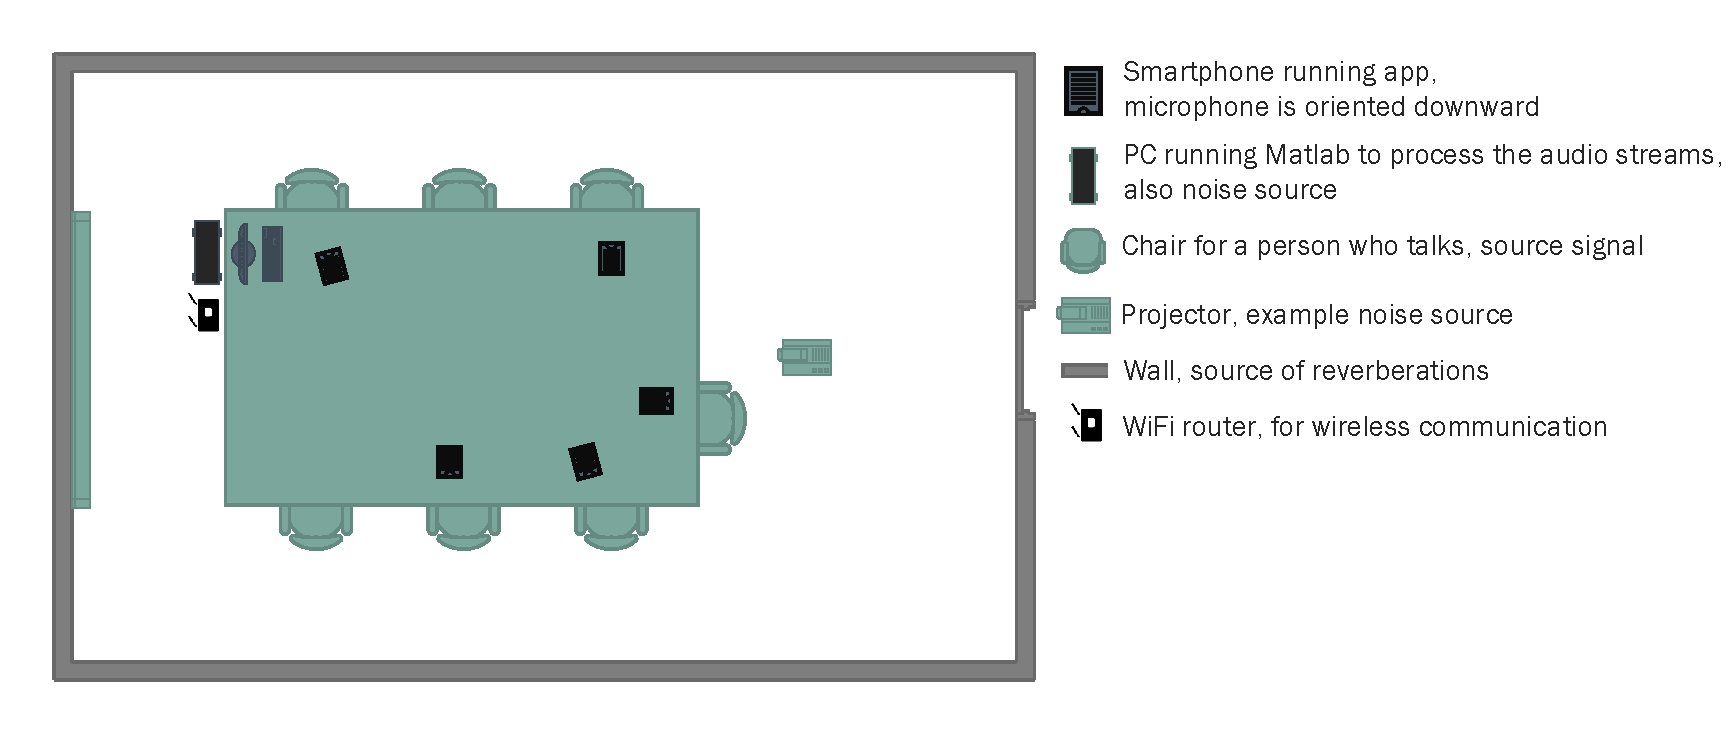
\includegraphics[width=15cm]{images/usage_scenario.pdf}
    \caption{An example usage scenario of the system in a conference call}
    \label{fig:SchemUsage}
\end{figure}

\section{Beamforming Algorithms}
\label{sec:intro_alg}
In this research, the delay-and sum beamformer and the minimum variance distortionless response (MVDR) beamformer are investigated. The MVDR beamformer is a very widely studied and used beamforming algorithm \citep{habetsspeech2010}, and is also used in commercially available arrays \citep{pentek2015}. The MVDR beamformer estimates the desired signal while minimizing the variance of the noise component of the formed estimate. The locations of the microphones are used to determine the direction of arrival (DOA). There are existing algorithms which can do source localization by using spectral estimation concepts and time-difference of arrival (TDOA) information \citep{brandstein2001}. Inaccuracies in the locations of the microphones degrade the performance of the MVDR beamformer significantly \citep{vanveen1988, ehrenberg2010}. Fortunately the microphone and source locations are known a priori in many cases \citep{himawan2011}. For this research perfect sound source localization (SSL) is assumed for both microphones and sources.

\section{Microphone Arrays}
\label{sec:intro_arrays}
Microphone arrays are a common way to improve the sound quality \citep{brandstein2001}. The diversity in the received signals is exploited by setting different gains to each microphone, depending on the location of the source and the interference. This is generally referred to as beamforming. Early designs were generally “fixed” beamformers like the delay-and-sum beamforming \cite{naylor2010speech}, adapting only to the location of the desired source. State of the art beamformers use statistical approaches which, in addition to the locations, also depend on assumptions about the acoustic composition of the signals \cite{gaubitch2014}. Iterative methods are also available which can adapt to specific noise and acoustic conditions \cite{griffiths1982,ba2007}. The latter methods have a considerably higher complexity \citep{kjellson2014sound}. \newline
A lot of research has been done into a class of algorithms known as robust MVDR beamformers \citep{ba2007,habets2010,martinez2015}. These algorithms improve upon previous work on two fronts, by extending the region where the source can be located and thus lowering the susceptibility to errors in the localization, and by including nonuniformity in the microphones directional response, known as microphone directivity.

\section{Microphone Directivity}
\label{sec:intro_directivity}
Real microphones may have distinct, directional responses. Experiments done by Ba et al. \citep{ba2007} show that the traditional MVDR beamforming algorithm and other existing algorithms perform well when omnidirectional microphones are used, but do not provide much enhancement when directional microphones are used. Simulations done by Martínez et al. \cite{gaubitch2014} show improvements of up to $6.1 dB$ in the segmental signal to noise ratio when using the measured directivity compared to assuming the microphones are omnidirectional \citep{martinez2015}. Aforementioned work used low cost smartphone microphones and the directivity pattern was measured in two dimensions. 
We will show in chapter \ref{chap:results} that including the directivity impulse response produced erratic results.
For the smartphones used in this work the directivities have been measured by our fellow team members \cite{BAP:RosalieTim}. This result is incorporated in the robust MVDR algorithm in section \ref{chap:design}. This has not been exploited much in the existing literature and in this thesis some of the challenges of implementing a realtime robust MVDR beamforming algorithm which adopts microphone directivity have been explored.

\section{Assessing Audio Quality}
\label{sec:intro_intelligibility}
In order to compare different beamformers, parameters and smartphone configurations an attempt has been made to write a realtime audio beamforming toolbox for \matlab which can interface with an Android app developed by our fellow team members \cite{BAP:RoySjoerd}. With this toolbox the impact of different aspects of beamforming on the quality estimators can be visualized in realtime. This enables rapid testing of different parameters and configurations. There are different quality estimators to analyze the performance of a beamformer. There are power related measures and intelligibility measures. Intelligibility is the degree to which speech can be understood and hence the corresponding measures can be evaluated to determine the effect of the beamformers on the speech intelligibility of the signals \cite{gerrits2014evaluation}.

\section{Reading Guide}
\label{sec:intro_reading}
This thesis is organized as follows. The last section (\ref{sec:intro_req}) of this introduction contains a schedule of requirements which was made at the start of the project. In chapter \ref{chap:problem}, the problem definition and observation model of this research will be defined. The research that has already been conducted in this topic will be discussed in section \ref{chap:related}. The design process is described in section \ref{chap:design}. The results are presented in section \ref{chap:results}. A discussion on these results is given in section \ref{chap:discussion}. A conclusion is drawn in section \ref{chap:conclusion}. Detailed results from the data analysis can be found in appendix \ref{app:res}.


\section{Requirements}
\label{sec:intro_req}
%\subsection{Introduction}
The aim of the system that will be implemented is to record audio, using smartphones, in a room with multiple audio sources and compare the performance of different beamforming algorithms. This comparison is done by showing different quantitative analyses related to a beamforming algorithm in a way that a user can compare the differences at a glance.

\subsection{Requirements concerning the intended use}
\begin{enumerate}
\item The system must have the possibility to either select local audio files for simulation or post-processing, or connect to smartphones for realtime calculations.
\item The noise has to be suppressed while maintaining the sound level of the source.
\item The noise source can be located anywhere, except at the source location.
\item The system must be able to switch between different types of beamformers.
\item The system must be able to compare the received audio from one of the smartphones before and after applying one of the beamformers.
\item The system must calculate and compare intelligibility metrics to determine the quality of the output for speech purposes.
\item The system must calculate and compare power related metrics to determine the quality of the output.
\item The system must be able record sound using smartphones.
\item The system must be able to play the beamformed audio over the speakers.
\item The system must be able to connect to the smartphones and handle the streaming data.
\item All of the requirements should be achieved in situations where the near-field assumptions hold.
\end{enumerate}

%After finishing recording, it has to be possible to save the output of each of the beamformers. 
%The system must be able to save the output of each of the beamformers.

% Consider following requirements
% It should be possible to filter at least 1 punctuated noise source by decreasing its power by at least 10 dB.

% It should be possible to aim a beam with a ’1’ response in an indicated target direction.

% Filtering has to be possible on the spectrum used for human speech, i.e. 300-3400 Hz.

\subsection{Requirements concerning the system}
\begin{enumerate}
\item The beamforming algorithms can be applied to real-time audio signals or previously recorded files.
\item For realtime beamforming, the communications between matlab and the smartphones will be monitored.
 For each smartphone individually the location, orientation and if the smartphone is placed face up or face down on the table can be entered.
\item Recording can be started and stopped by pressing a start/stop button.
\item The different beamformers can be turned on or of by ticking the corresponding box.
\item Each of the different kinds of intelligibility and power related calculations can be selected or deselected.
\item While recording, the location(s) of the source(s) and microphone(s) will be plotted on the screen in 3D.
\item After recording, the relevant data can be saved to an audio file, including sufficient data labels such as locations to make post-processing possible.
\item In the non realtime case, the user will be able to select a time frame which will be beamformed and over which the intelligibility and power related measures will be computed.
\end{enumerate}